\documentclass[a4paper,12pt]{report}

\usepackage{graphicx}
\usepackage[utf8]{inputenc}
\usepackage[italian]{babel}
\usepackage{geometry}
\usepackage{setspace}
\usepackage{titlesec}
\usepackage{fontspec}
\usepackage{subfig}
\usepackage{tikz}
\usepackage{caption}
\usepackage{listings}
\usepackage{enumitem}
\usepackage{float}



\captionsetup{
  font=small, % Imposta il font delle didascalie come "small" (piccolo)
  justification=centering, % Allinea le didascalie al centro
  singlelinecheck=false, % Permette alle didascalie di occupare più righe se necessario
  skip=5pt % Aggiunge uno spazio verticale di 5pt tra la figura e la didascalia
}

\setmainfont{Calibri}

\geometry{
  a4paper,
  left=4.5cm,
  right=3cm,
  top=4cm,
  bottom=4cm,
}

\lstset{
    language=Python,
    basicstyle=\ttfamily\small,
    keywordstyle=\color{blue},
    commentstyle=\color{green!40!black},
    stringstyle=\color{orange},
    showstringspaces=false,
    breaklines=true,
    frame=single,
    numbers=left,
    numberstyle=\tiny,
    captionpos=b,
    lineskip=1pt
}

\titleformat{\section}
  {\fontsize{14}{16}\bfseries}
  {\thesection}
  {1em}
  {}

\titleformat{\subsection}
  {\fontsize{12}{14}\bfseries}
  {\thesubsection}
  {1em}
  {}

\linespread{1.5}
\setlength{\parindent}{0pt}

\begin{document}
\selectlanguage{italian}

\begin{titlepage}
\centering

\textbf{\large Università degli Studi di Bari} \\
\vspace{0.5cm}
\textbf{\large Dipartimento di Informatica} \\
\vspace{2cm}

\includegraphics[width=40mm,scale=0.5]{assets/images/logo.png} \\
\vspace{2cm}
\textbf{\large Tesi di Laurea Triennale in Informatica e Tecnologie per la Produzione del Software} \\
\vspace{1cm}
\textbf{\LARGE Progettazione sistema SPIR} \\
\vspace{1cm}
\textbf{\large Autore:} \\
\textbf{Antonio Ricciardi} \\
\vspace{0.3cm}
\textbf{\large Relatore:} \\
\textbf{Giovanni Dimauro} \\
\vspace{0.3cm}
\textbf{\large Correlatori:} \\
\textbf{Rosalia Maglietta} \\
\textbf{Carla Cherubini} \\
\vfill
\textbf{\large Anno Accademico 2022/2023} % Inserisci l'anno accademico corretto
    
\end{titlepage}

\tableofcontents
\chapter{Introduzione}
  Fondamentale implementare la fotoid
  \section{Stato dell'arte}
    \subsection{Elaborazione delle immagini}
      La manipolazione e l'elaborazione delle immagini svolgono un ruolo fondamentale in numerosi settori, tra cui la visione artificiale, la grafica computazionale e l'analisi di immagini biomediche. 
      In quest'ambito, gli operatori morfologici e logici giocano un ruolo chiave nella modifica e nell'estrazione di informazioni significative da immagini digitali. \\
      Gli operatori morfologici sono basati sulla teoria della morfologia matematica e vengono utilizzati per la manipolazione di forme geometriche all'interno di un'immagine. \\
      Essi consentono di eseguire operazioni come l'erosione, la dilatazione, l'apertura e la chiusura, che possono essere utilizzate per rimuovere rumore, riempire buchi o separare oggetti connessi. \\
      L'erosione riduce le regioni di colore o intensità nell'immagine, mentre la dilatazione le amplia. L'apertura è una combinazione di erosione seguita da dilatazione e viene utilizzata per rimuovere piccoli oggetti o dettagli indesiderati. La chiusura, al contrario, consiste in una dilatazione seguita da erosione ed è utile per riempire buchi o connettere regioni separate.
      Parallelamente agli operatori morfologici, gli operatori logici sono ampiamente utilizzati per combinare e confrontare immagini. Gli operatori logici fondamentali includono l'AND, l'OR e il NOT, che consentono di creare maschere o combinare informazioni da diverse immagini. \\
      Ad esempio, l'operatore AND può essere utilizzato per identificare le regioni comuni tra due immagini, mentre l'operatore OR può essere impiegato per unire due immagini sovrapposte in una sola immagine risultante. \\
      L'operatore NOT, invece, inverte i valori di pixel di un'immagine, consentendo di creare effetti speciali o evidenziare determinate regioni.
    \subsection{Feature Extraction}
    \subsection{Object Segmentation}
    \subsection{User Interface}
    \subsection{SPIR}
  \section{Obiettivi}

\chapter{Metodi}
  \section{Porting del sistema SPIR}
    In una prima fase di analisi di SPIR (MATLAB) si nota che l'interazione è confinata
    a linea di comando (CLI), in ottica di offrire le funzionalità di SPIR a una più ampia
    fascia di utenza, mantendo anche la possibilità di usufruire del codice sorgente 
    da parte di utenti più esperti si è optato per una implementazione basata su client/server,
    in particolare slegando le componenti di interazione e logica del sistema si ha la possibilità
    di utilizzare le tecnologie più apporpriate a seconda del contesto, per poi mettere in comunicazione le 
    varie componenti.
    \subsection{Riscrittura dell'algoritmo originale (MATLAB) in Python}
      Lo sviluppo si è concentrato inizialmente sulla riscrittura delle funzionalità principali di SPIR,
      come linguaggio è stato scelto Python per i seguenti motivi:
      \begin{itemize}
        \item Vasta gamma di librerie per la manipolazione di immagini disponibili.
        \item Utilizzo di OpenCV per l'elaborazione delle immagini.
        \item Buona diffusione in ambito scientifico.
        \item Supporto attivo dalla community di sviluppatori.
      \end{itemize}

      La prima funzionalità presa in analisi per il porting è stata l'estrazione delle maschere dalle immagini,
      di fondamentale importanza al fine di ottimizzare l'area di estrazione delle features, l'estrazione delle maschere viene fatta
      nel metodo 
      \begin{verbatim}
prepare_images_vlfeat.m
      \end{verbatim}
      \begin{figure}
        \centering
        
        \begin{minipage}{0.35\textwidth}
          \centering
          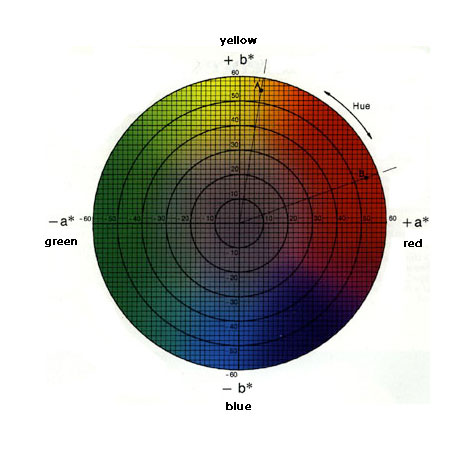
\includegraphics[width=\textwidth]{assets/images/cielab2.jpg}  
          \caption{Spazio colore CIELAB in 2D}
        \end{minipage}
        \begin{minipage}{0.35\textwidth}
          \centering
          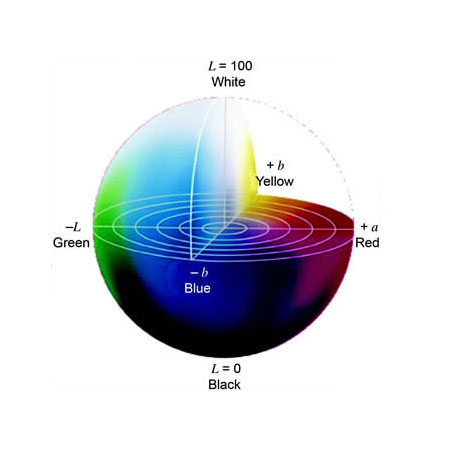
\includegraphics[width=\textwidth]{assets/images/cielab1.jpg}   
          \caption{Spazio colore CIELAB in 3D}
        \end{minipage}
      \end{figure}

      L'immagine viene convertita nello spazio colore Cielab, è uno spazio \\
      colore-opponente con la dimensione L per la luminosità e a e b per le dimensioni colore-opponente,
      basato sulle coordinate dello spazio colore non lineare compresso CIE XYZ.
      La luminosità è calcolata usando la radice cubica della luminanza relativa. 
      Lab include tutti i colori percepibili, perciò include completamente i gamut degli 
      spazi colore RGB e CMYK ed è indipendente dal dispositivo che li rappresenta.
      
      Come nella versione originale il primo passo è convertire l'immagine da RGB a CIELAB, 
      a differenza di matlab OpenCV utilizza il formato BGR, ovvero il vettore dei colori per ogni pixel è invertito,
      dall'immagine convertita in spazio colore CIELAB si estrae il canale B dall'immagine questo permette di mettere in evidenza 
      le aree blu dell'immagine così da isolare la parte di mare presente nello sfondo delle foto.
      \newpage
      La sogliatura di Otsu, chiamata anche metodo di Otsu, è un algoritmo utilizzato per determinare automaticamente il valore di soglia ottimale per la segmentazione di un'immagine in bianco e nero.
      L'obiettivo della sogliatura è quello di separare i pixel dell'immagine in due classi, generalmente il primo piano (oggetti di interesse) e lo sfondo.
      \begin{figure}
        \centering
        
        \begin{minipage}{0.25\textwidth}
          \centering
          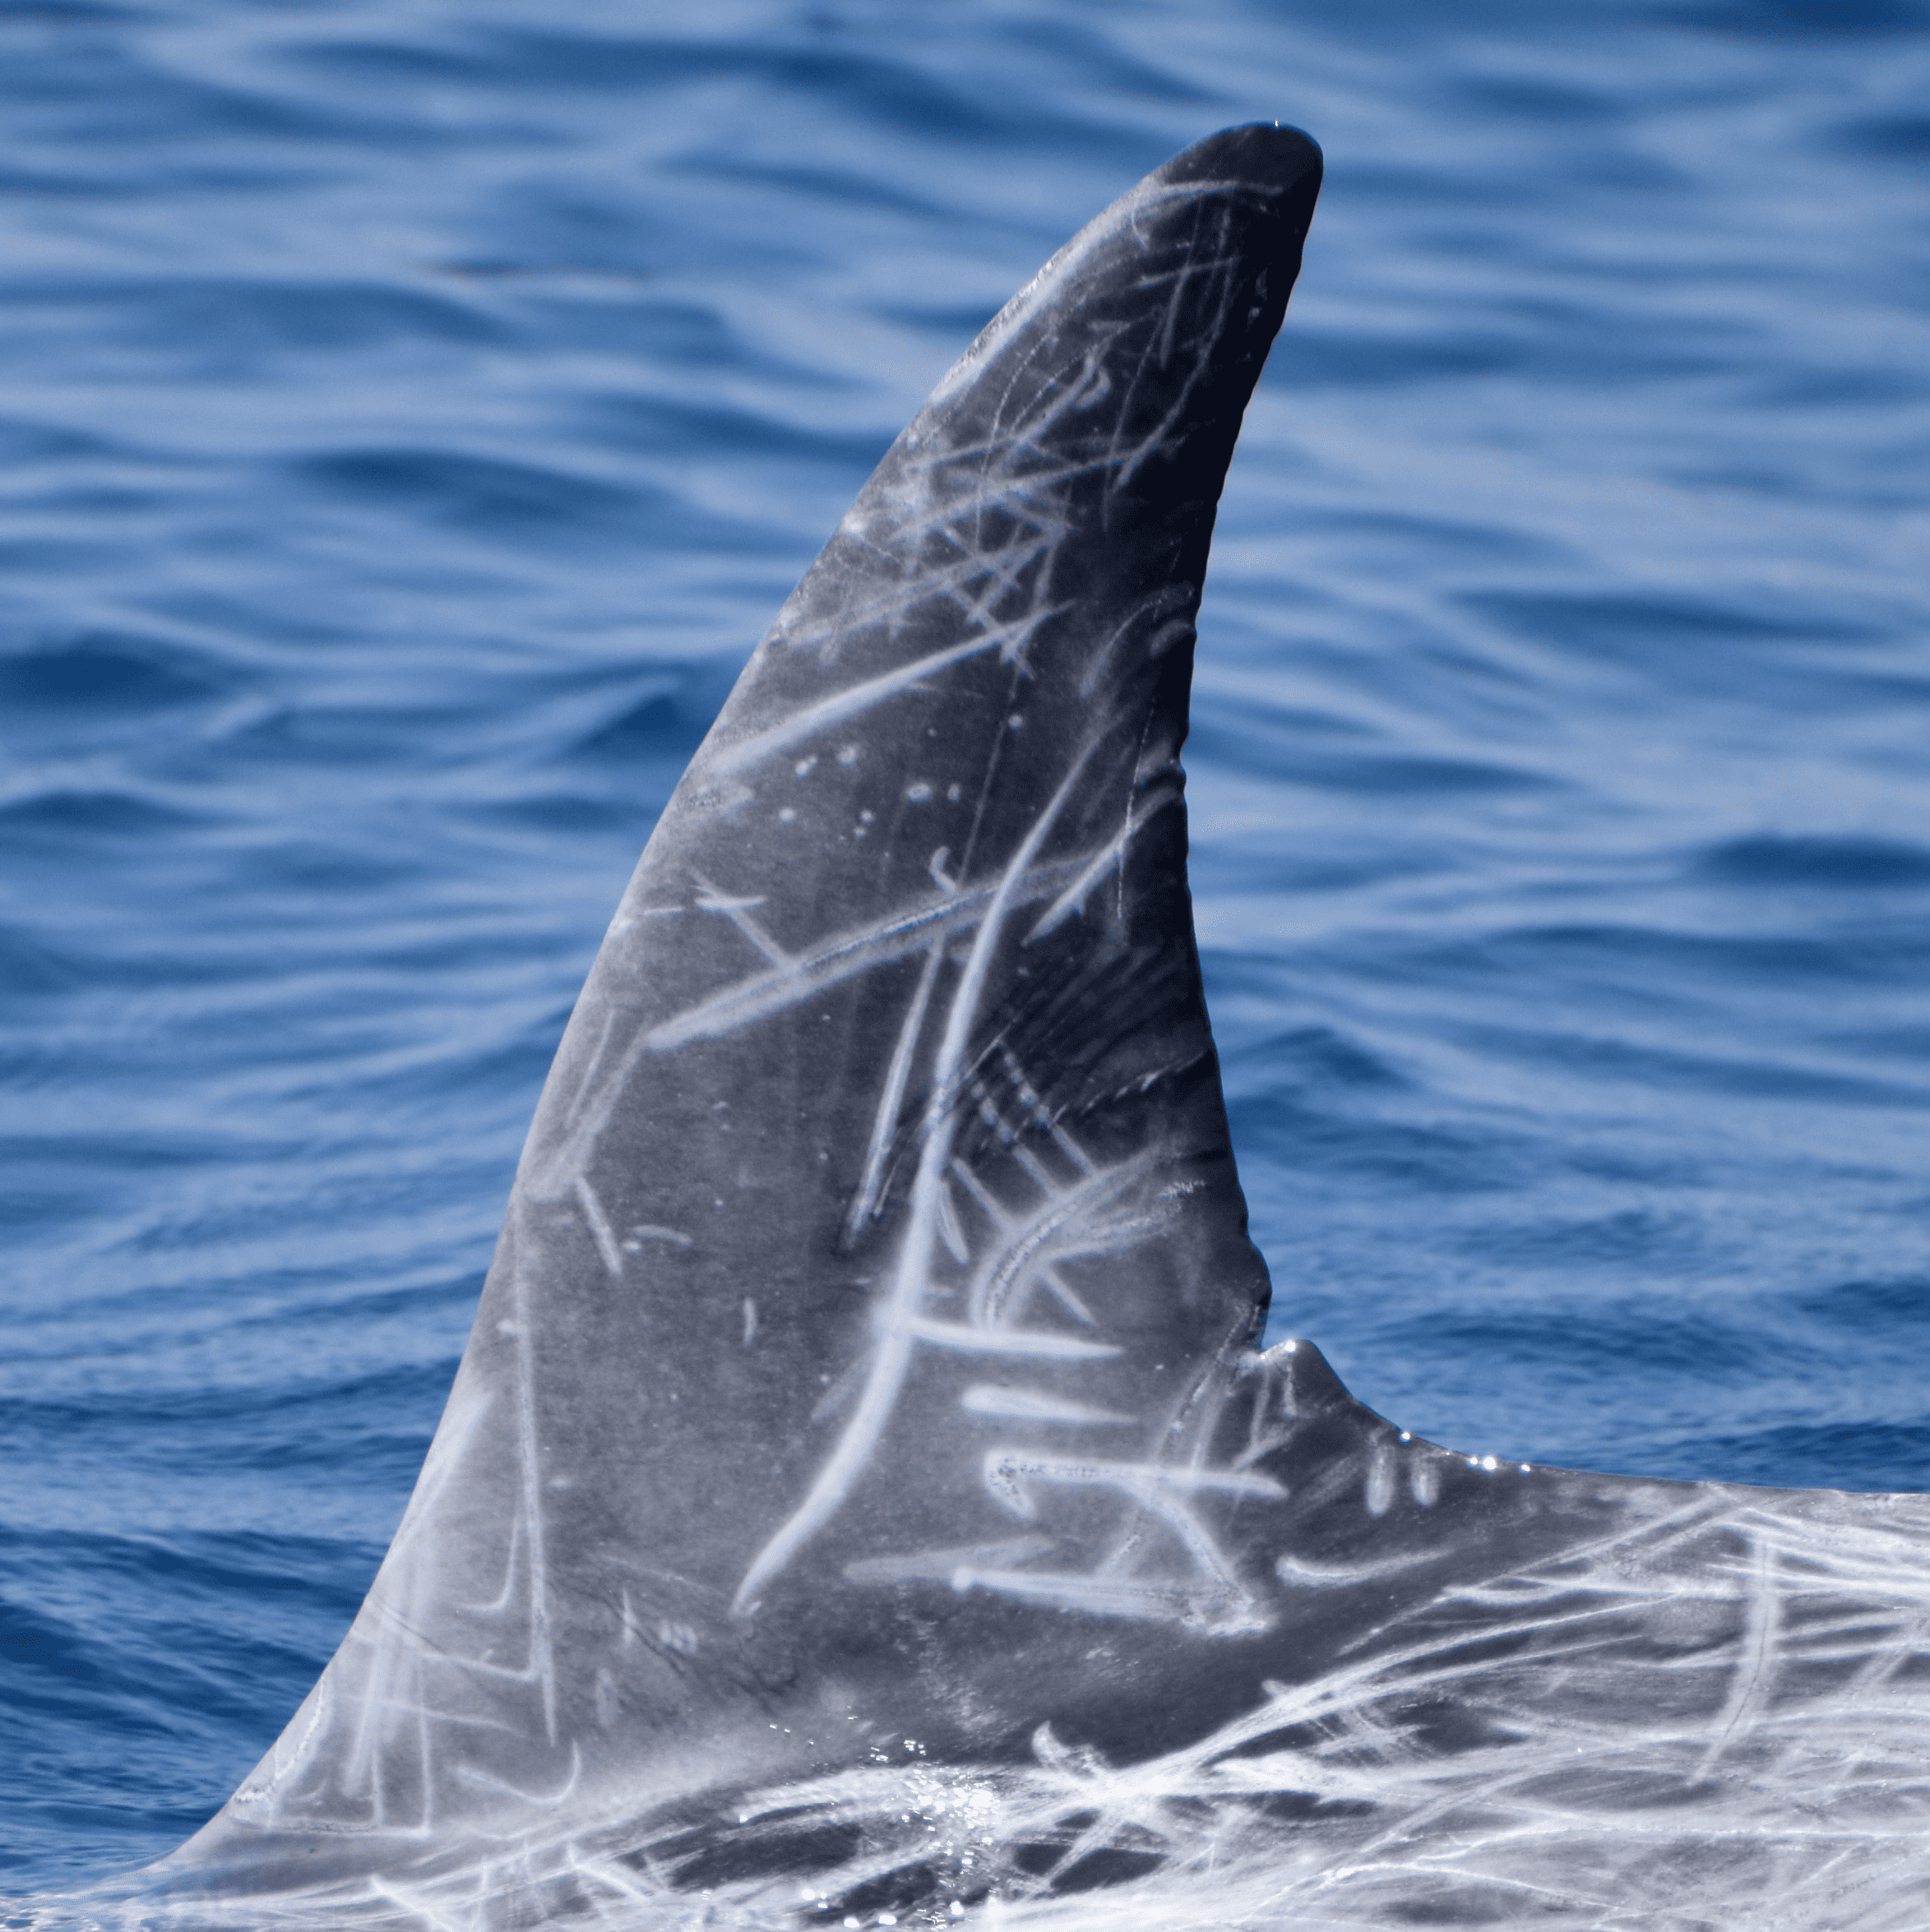
\includegraphics[width=\textwidth]{assets/images/fin_extraction/test_original.png}  
          \caption{Immagine originale}
        \end{minipage}
        \begin{minipage}{0.25\textwidth}
          \centering
          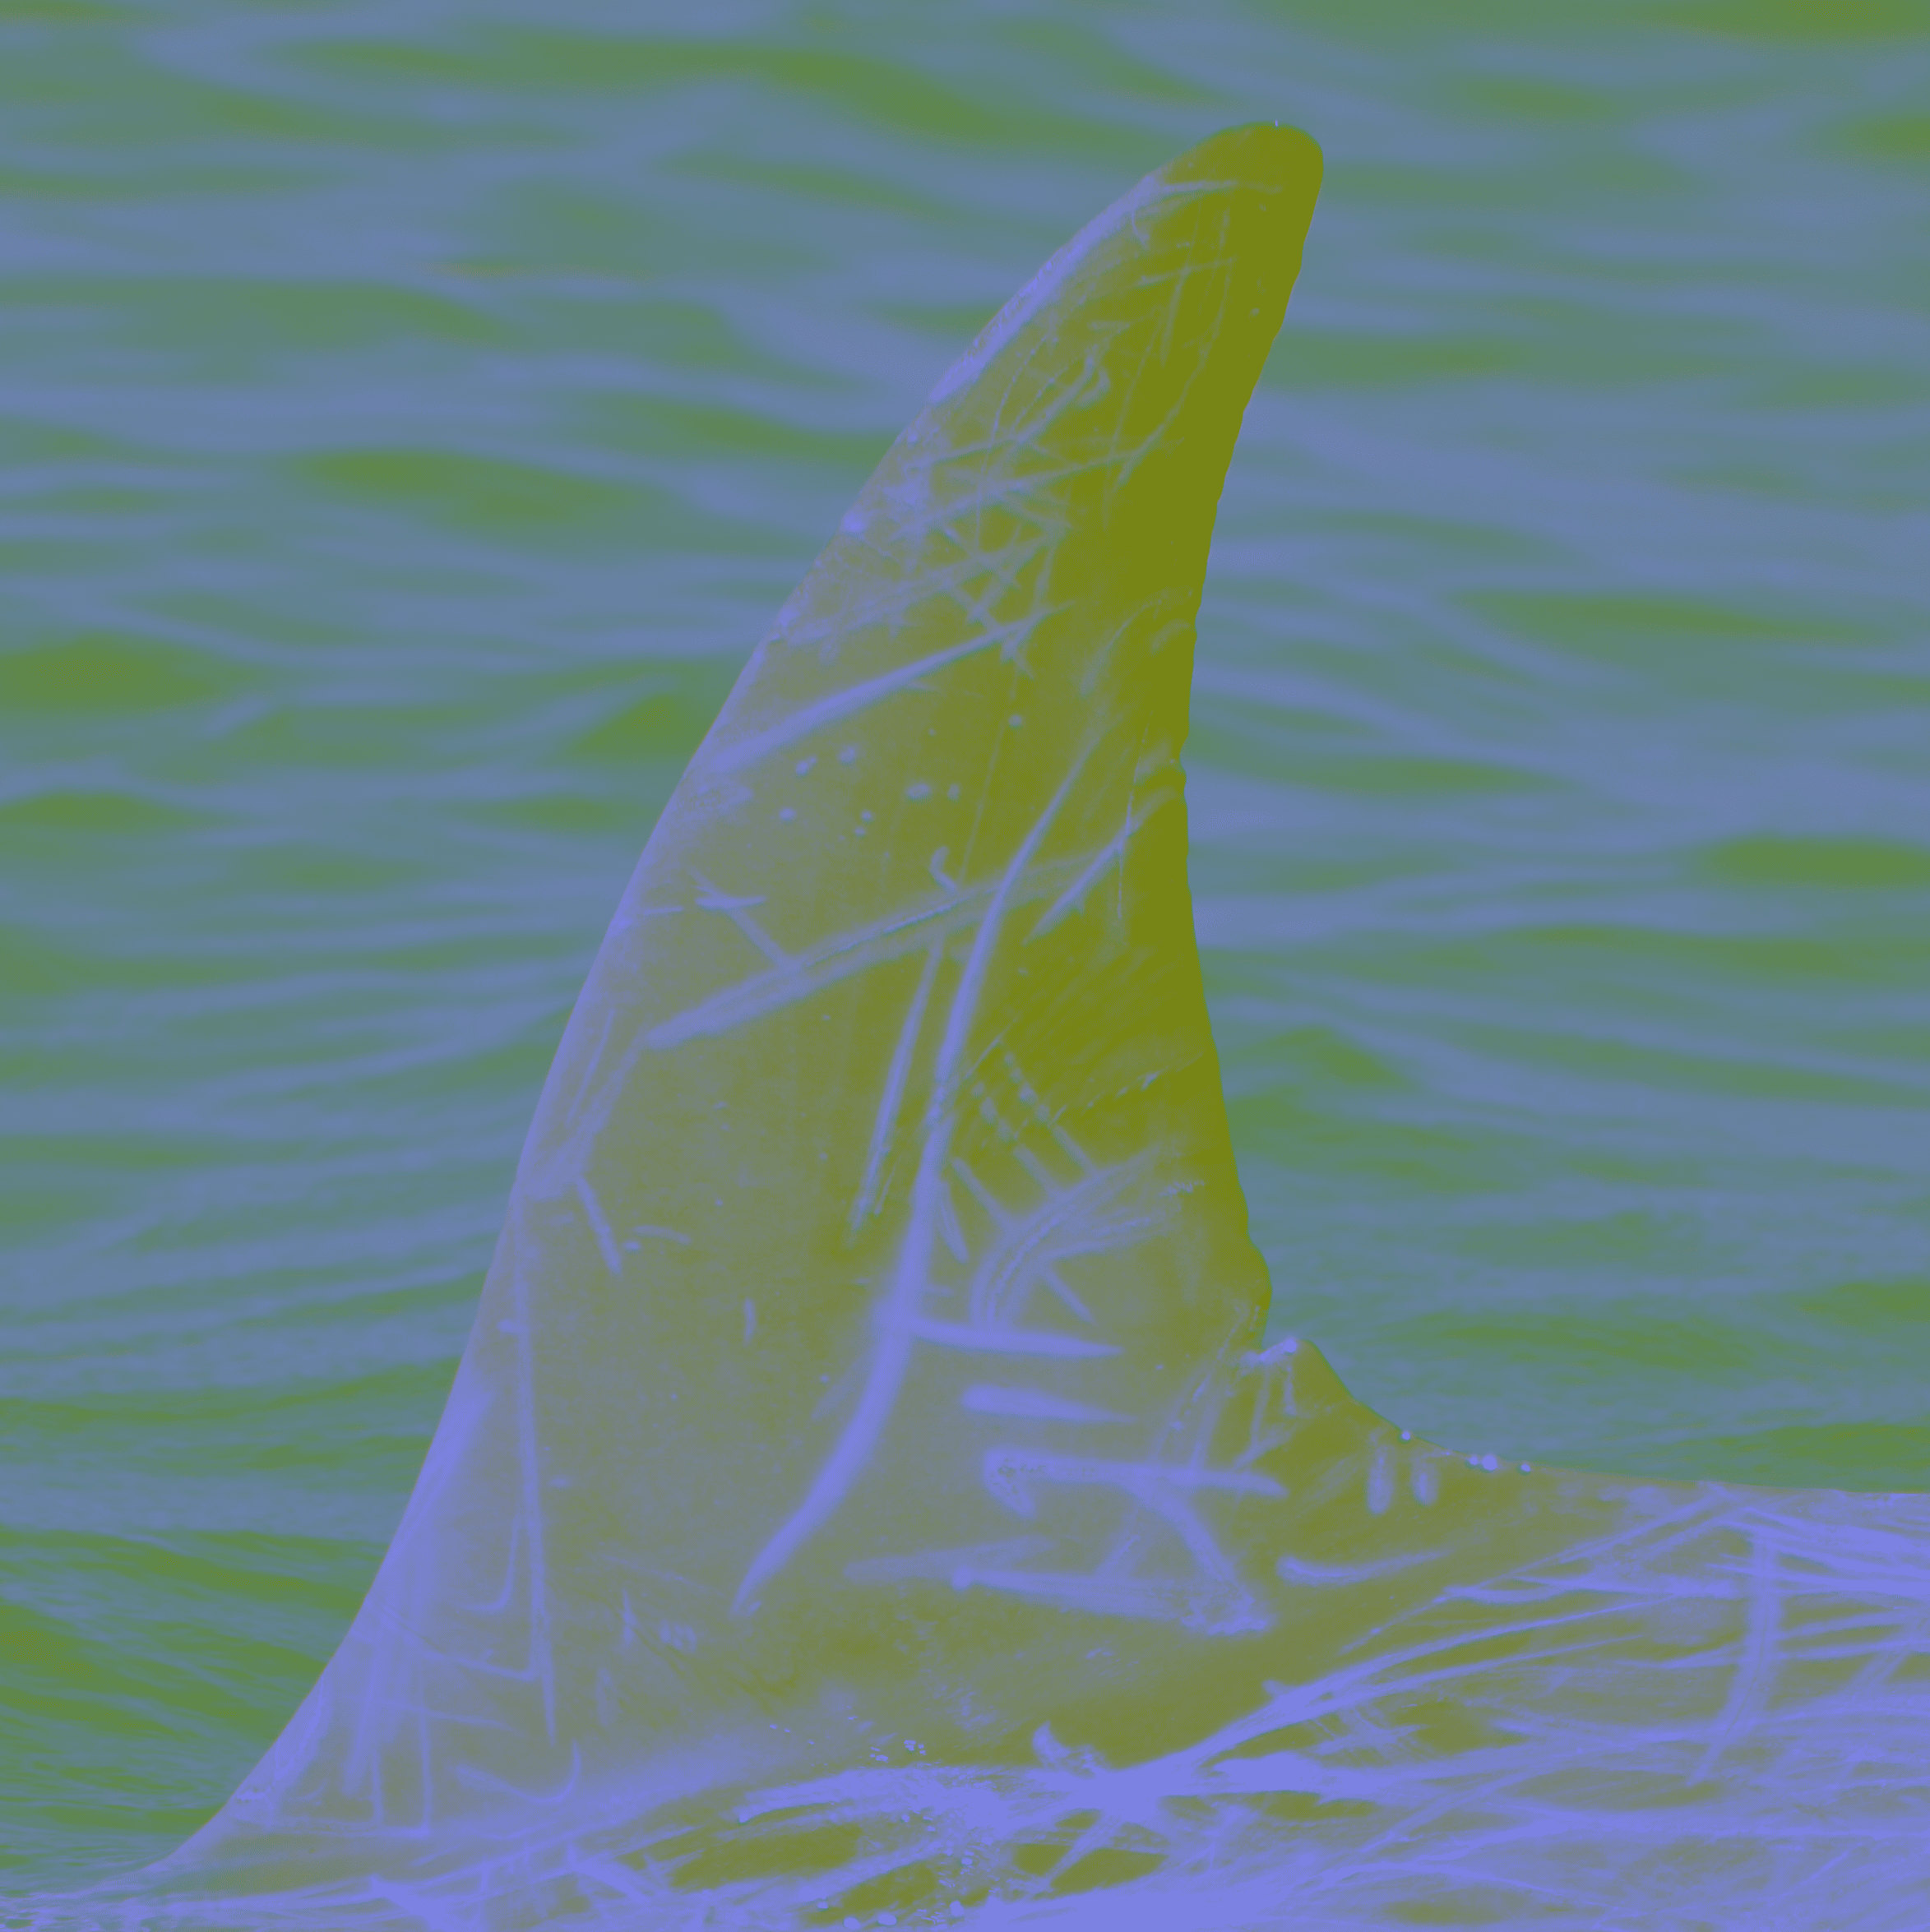
\includegraphics[width=\textwidth]{assets/images/fin_extraction/test_lab.png}   
          \caption{Immagine CIELAB}
        \end{minipage}
        \begin{minipage}{0.25\textwidth}
          \centering
          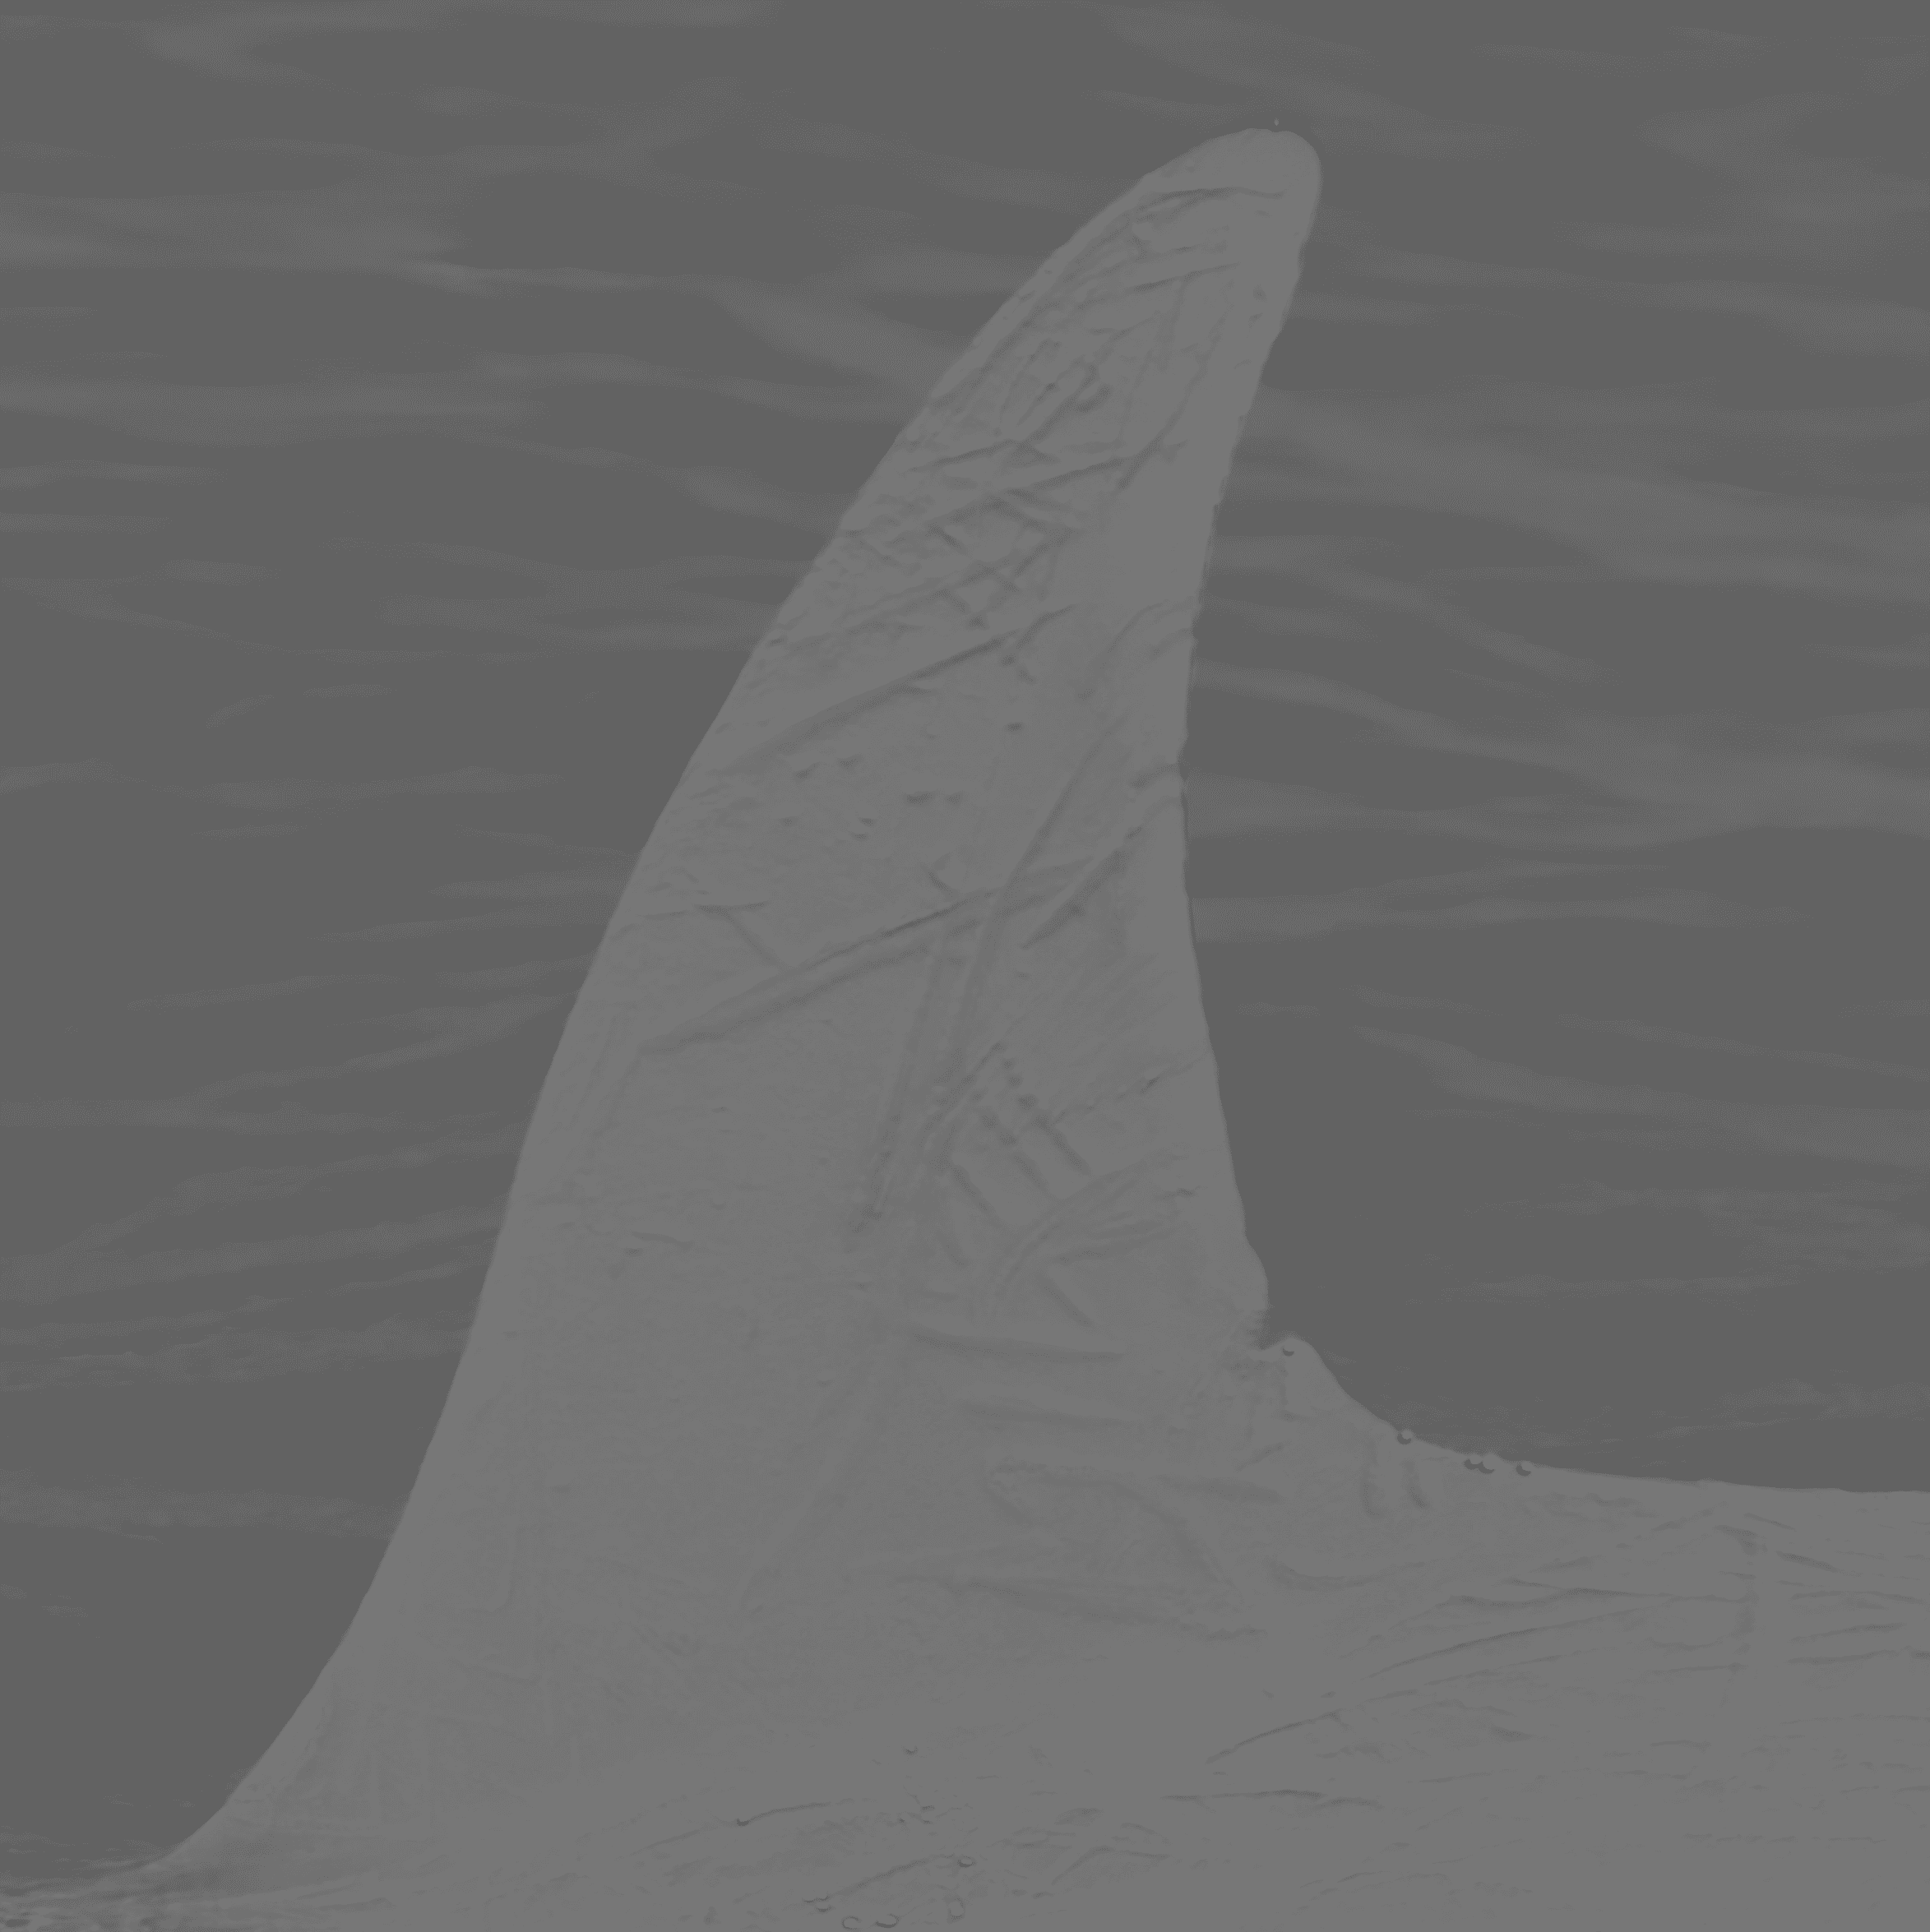
\includegraphics[width=\textwidth]{assets/images/fin_extraction/test_b.png}  
          \caption{Canale B estratto}
        \end{minipage}

        
      \end{figure}

      \begin{lstlisting}
#Caricamento immagine originale
image = cv2.imread("BEN_180713_4.png")

#Conversione immagine in spazio colore CIELAB
im_lab = cv2.cvtColor(image, cv2.COLOR_BGR2LAB)

#Estrazione del canale B
b = im_lab[:,:,2]

# Applico il metodo di Otsu al canale B
thr_b, _ = cv2.threshold(b, 0, 255, cv2.THRESH_BINARY + cv2.THRESH_OTSU)
      \end{lstlisting}

        L'algoritmo di Otsu calcola la soglia ottimale in base all'istogramma dei livelli di grigio dell'immagine.
        L'istogramma rappresenta la distribuzione dei valori di grigio presenti nell'immagine.
        \newpage
        L'obiettivo è trovare la soglia che massimizza la varianza tra le due classi (primo piano e sfondo), 
        considerando anche la distribuzione dei pixel di ciascuna classe.
        In altre parole, si cerca la soglia che massimizza la separazione tra i due gruppi di pixel.

      \begin{figure}
        \centering
        \begin{minipage}{0.25\textwidth}
          \centering
          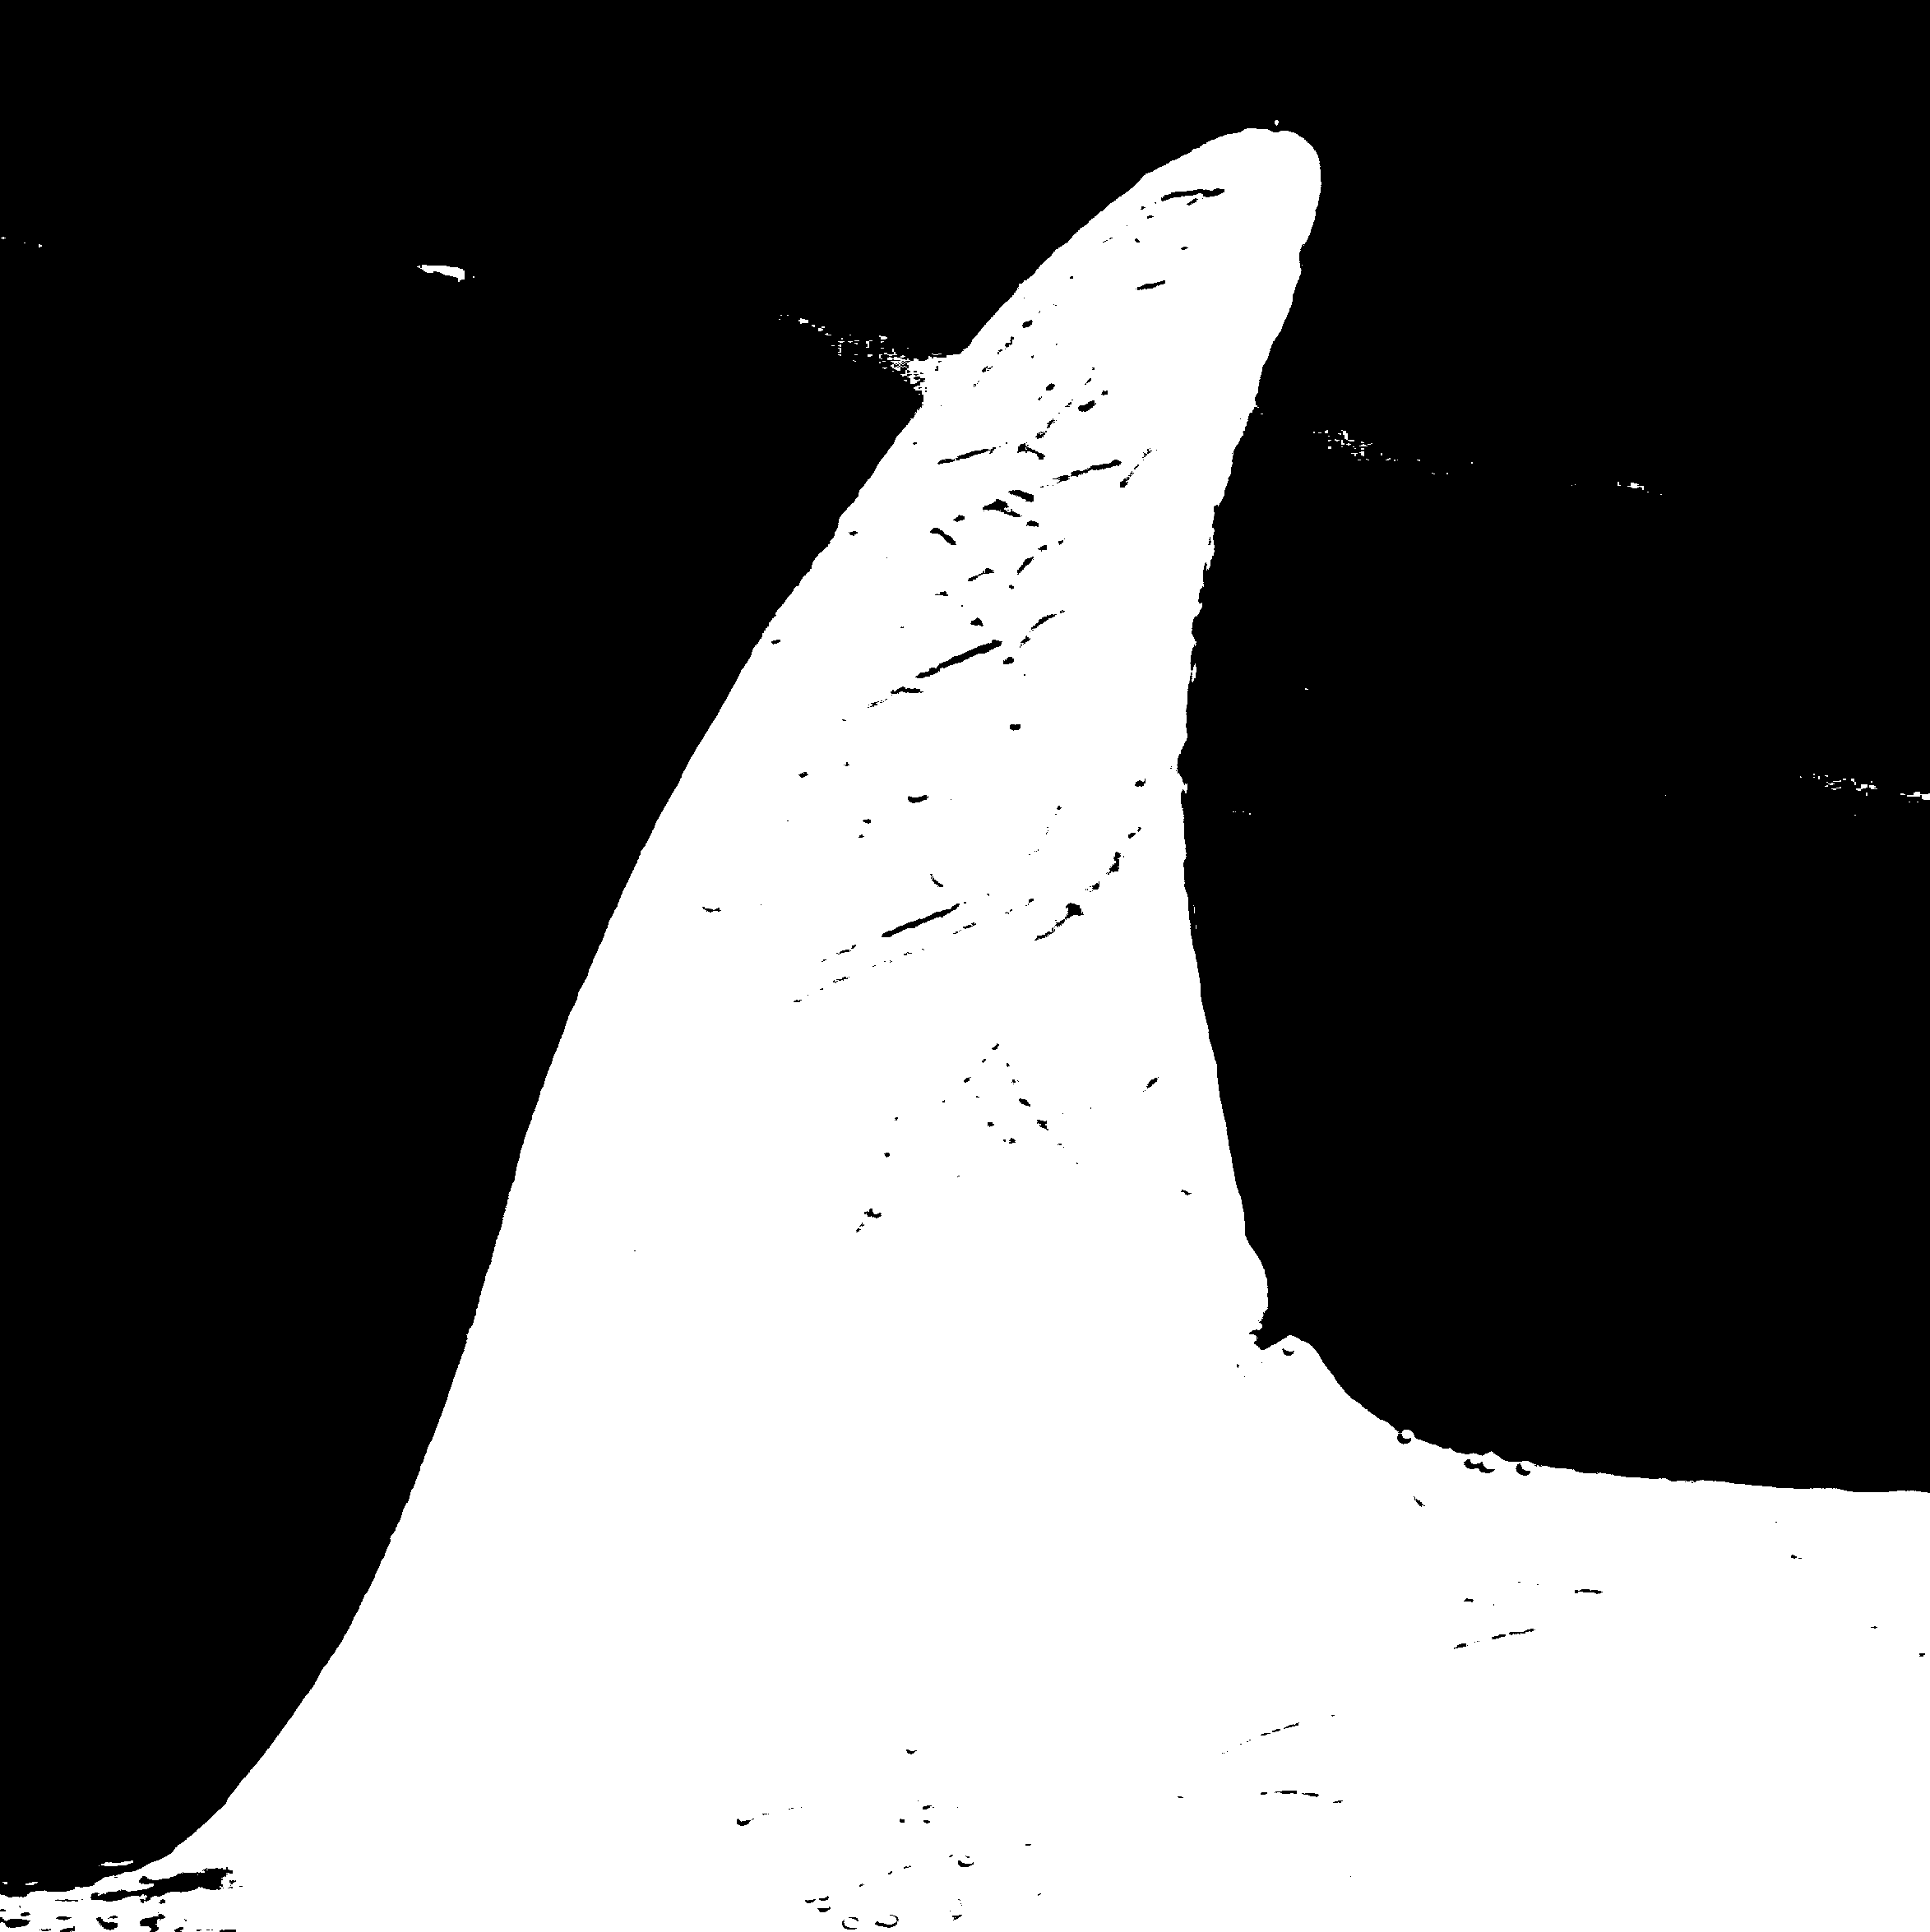
\includegraphics[width=\textwidth]{assets/images/fin_extraction/test_thr_b.png}   
          \caption{Metodo OTSU}
        \end{minipage}
        \begin{minipage}{0.25\textwidth}
          \centering
          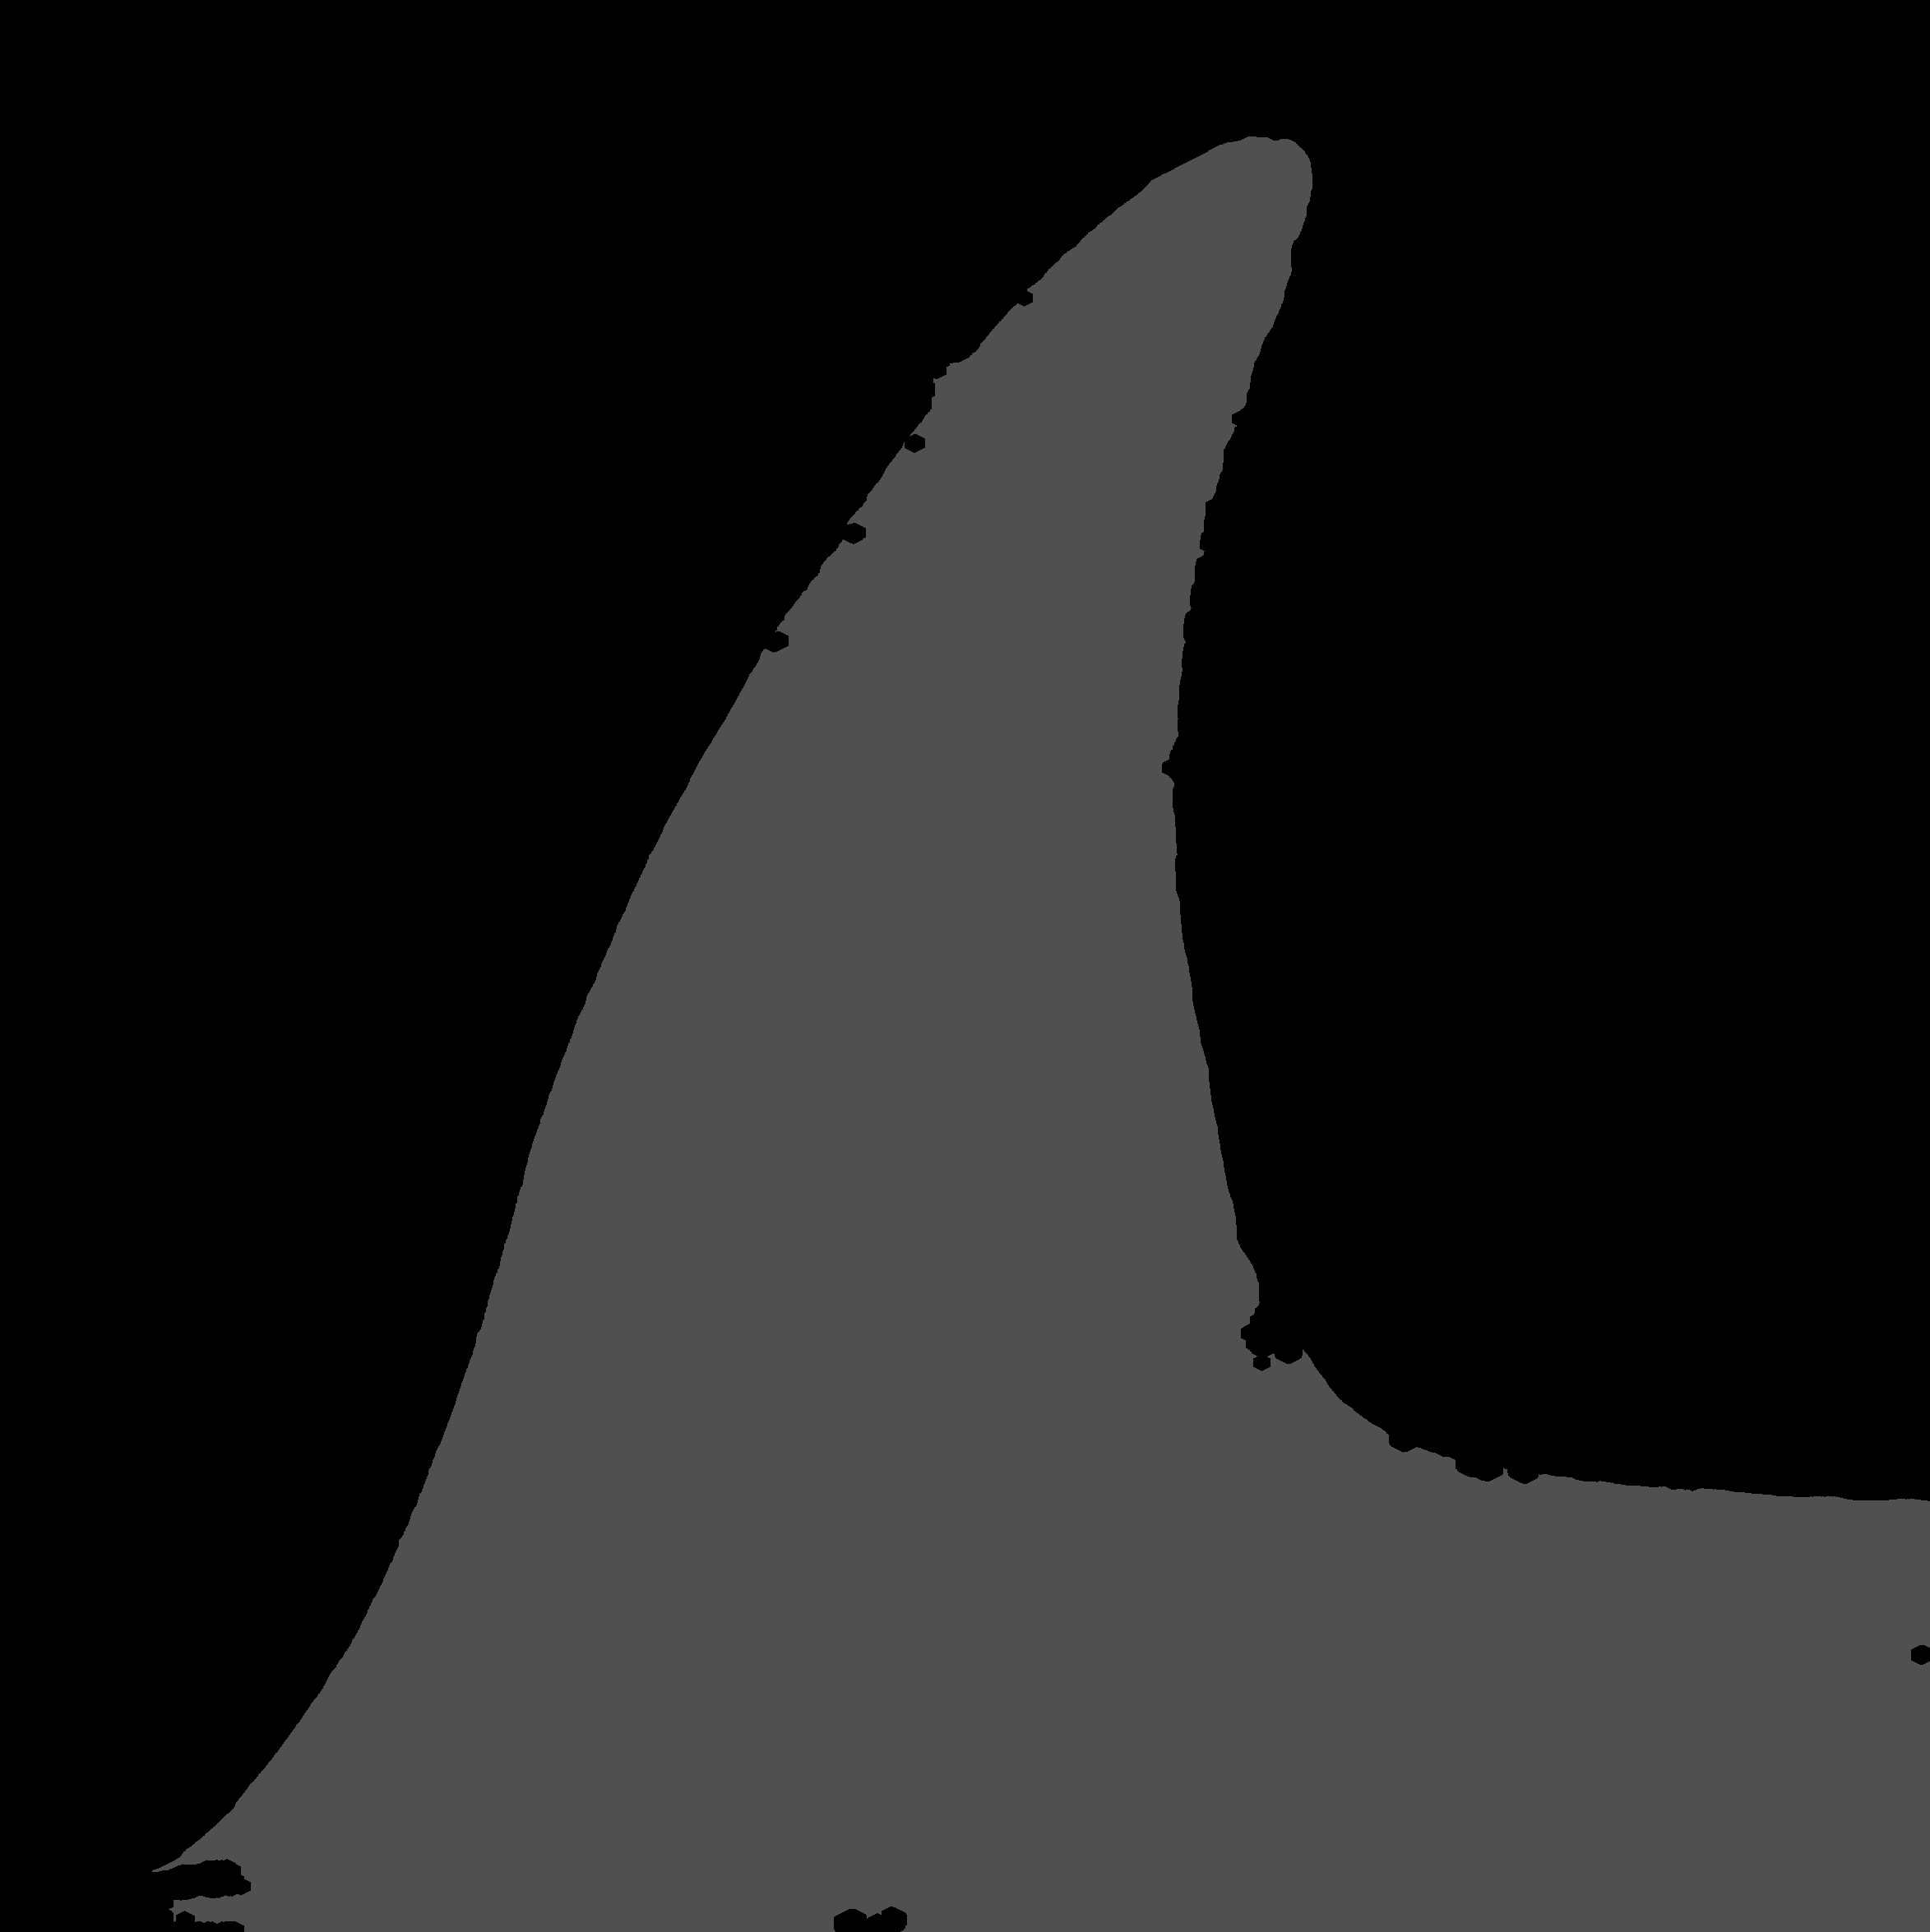
\includegraphics[width=\textwidth]{assets/images/fin_extraction/test_mask1.png}  
          \caption{Operatori morfologici e pulizia}
        \end{minipage}
        \begin{minipage}{0.25\textwidth}
          \centering
          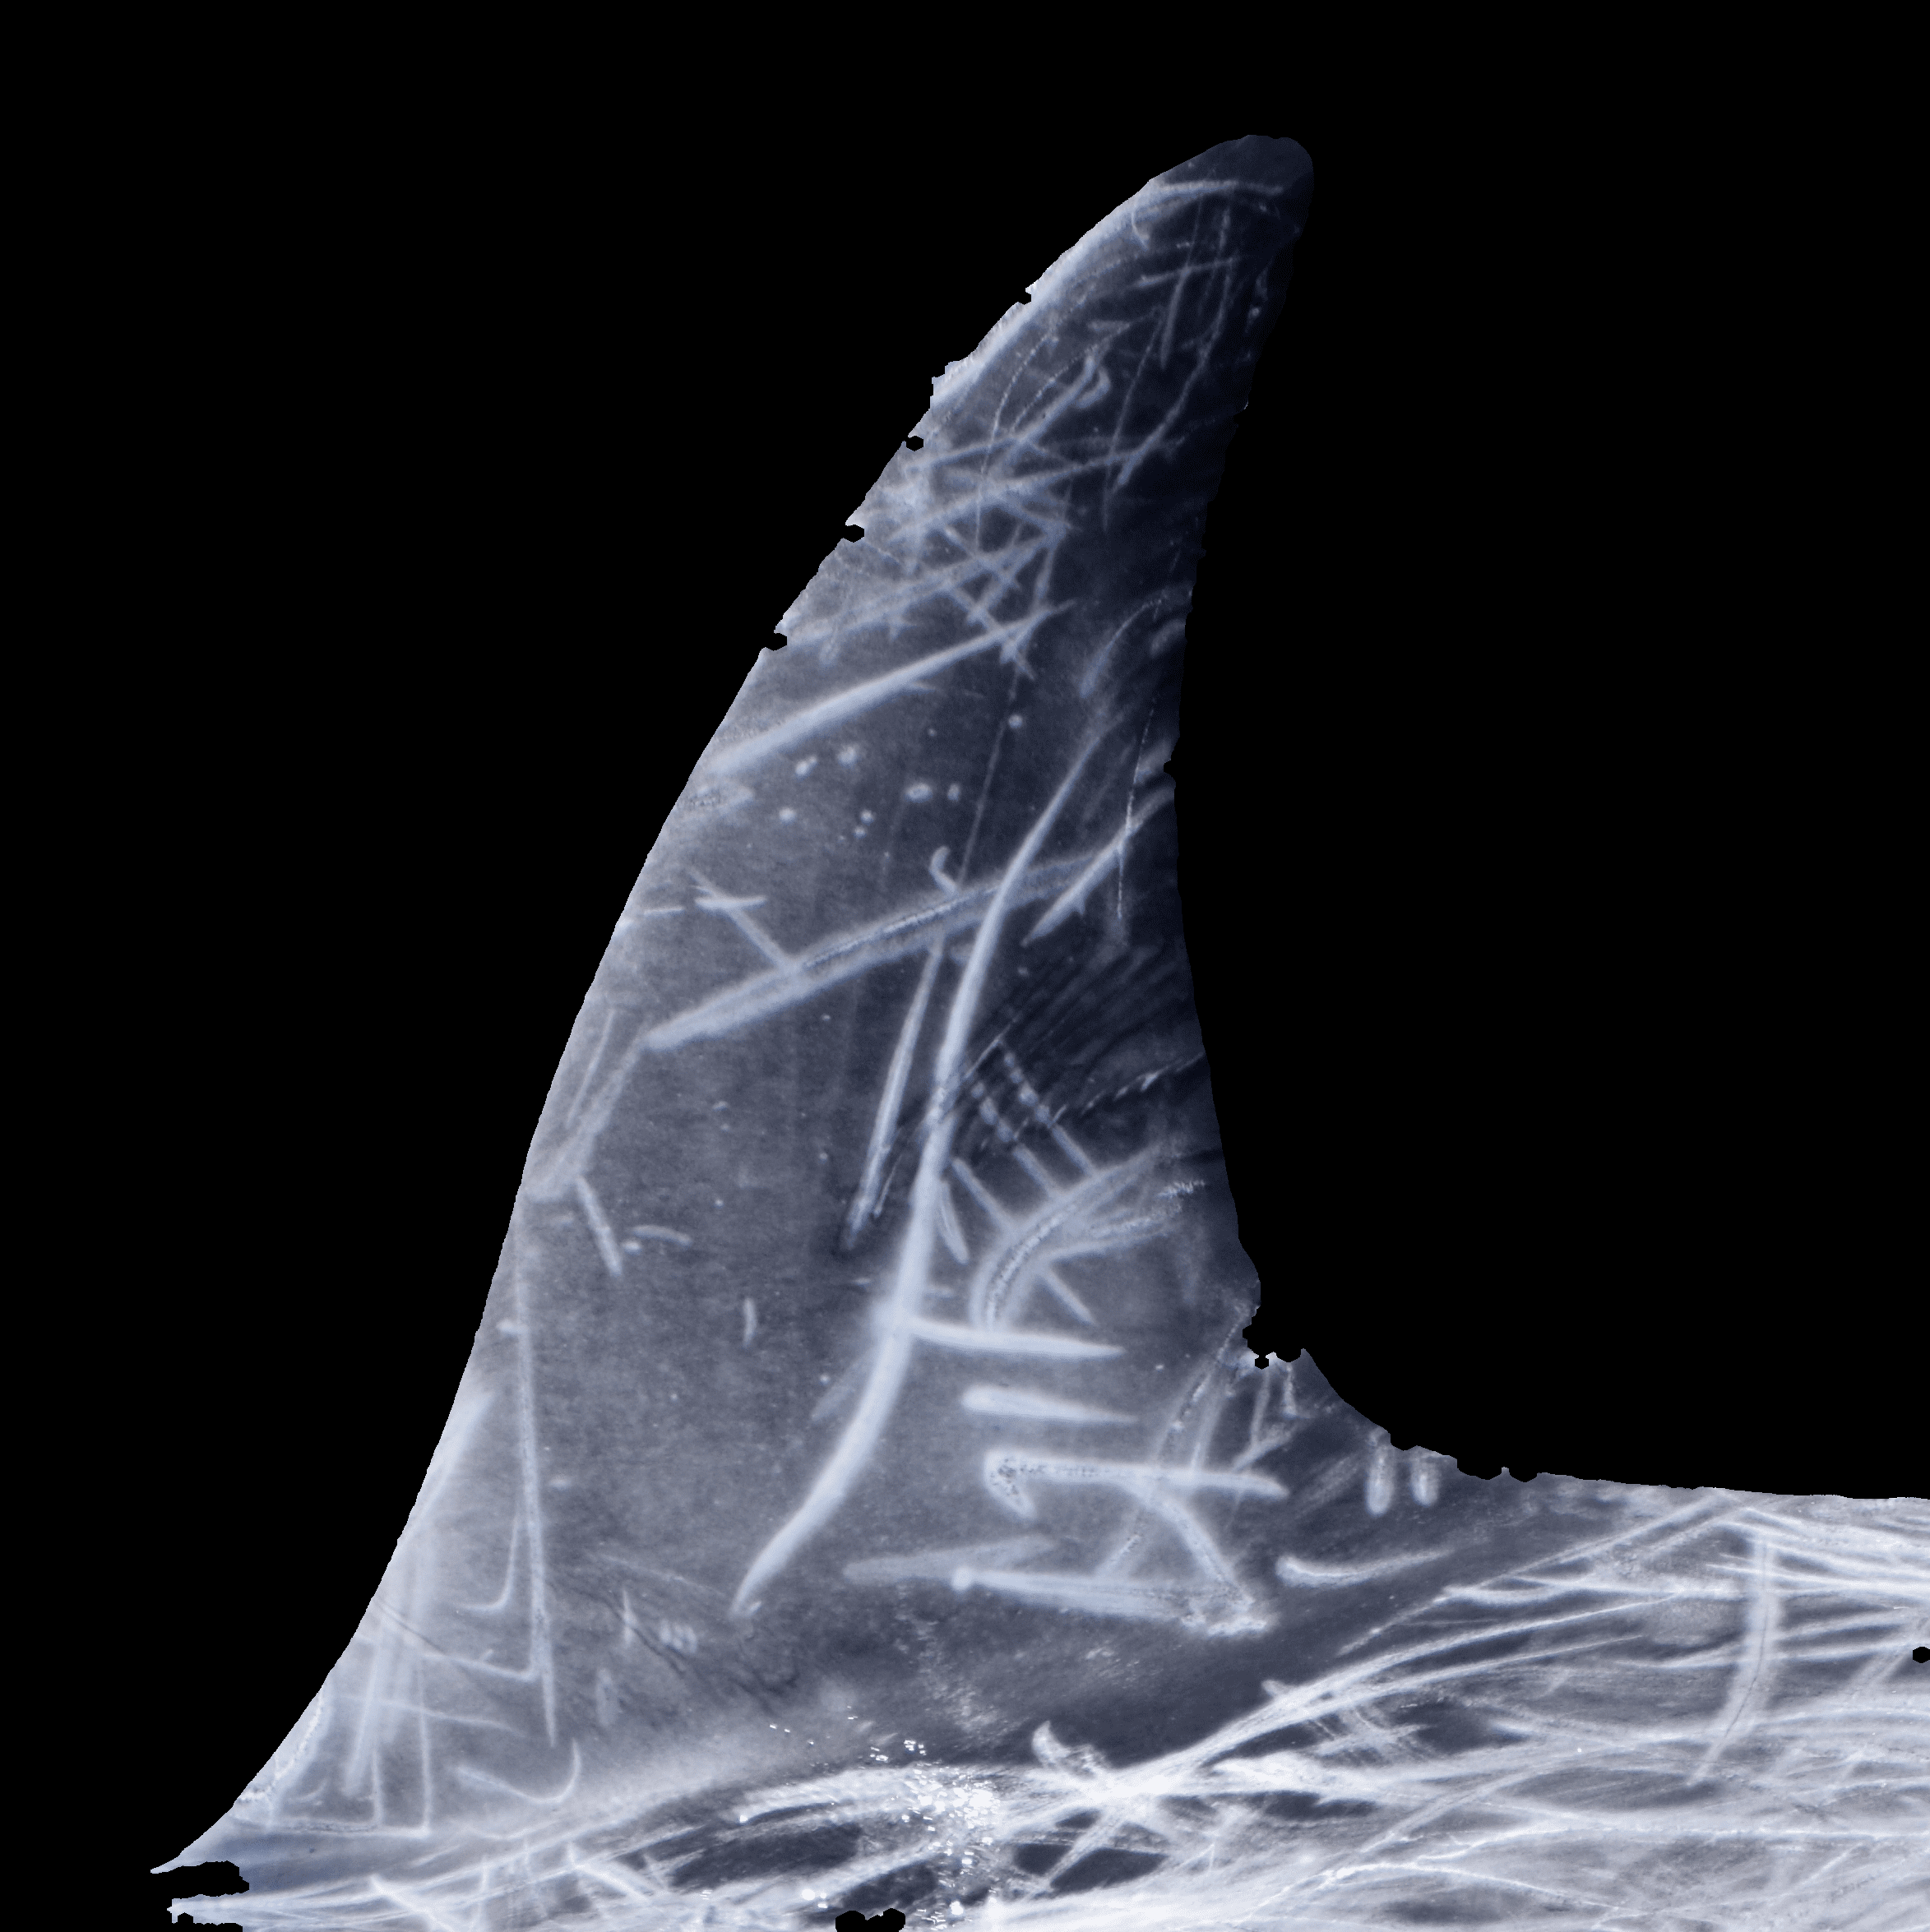
\includegraphics[width=\textwidth]{assets/images/fin_extraction/test_out.png}   
          \caption{Pinna estratta}
        \end{minipage}
        \begin{flushleft}
          
        \end{flushleft}
      \end{figure}
      Una volta prodotta la prima maschera grazie al metodo OTSU, 
      si passa all'eliminazione dei buchi mediante l'utilizzo di operatori
      morfologici e alla rimozione di segmenti slegati dall'area della pinna.
      Nello specifico gli operatori morfologici utilizzati per l'elimiazione dei buchi sono stati:
      \begin{itemize}
        \item Dilatazione (Dilation): L'operazione di dilatazione viene utilizzata per \\espandere le regioni di pixel bianchi nell'immagine. In sostanza, ogni pixel bianco nell'immagine di input viene "gonfiato" e riempito con pixel bianchi circostanti. Ciò ha l'effetto di aumentare le dimensioni dell'oggetto o delle strutture bianche nell'immagine. L'operazione di dilatazione è utile per riempire eventuali buchi o lacune all'interno delle regioni, connettere regioni separate o aumentare la dimensione degli oggetti.
        \item Chiusura (Closing): L'operazione di chiusura combina l'erosione seguita dalla dilatazione per rimuovere piccoli buchi o aree isolate all'interno delle regioni bianche dell'immagine. Inizialmente, l'operazione di erosione viene applicata per ridurre le dimensioni delle regioni bianche e rimuovere dettagli indesiderati. Successivamente, l'operazione di dilatazione viene applicata per riempire i buchi e ricongiungere le regioni vicine che potrebbero essere state separate durante l'erosione. L'operazione di chiusura è utile per ridurre il rumore, migliorare la coerenza delle regioni e completare le forme degli oggetti.
      \end{itemize}
      \begin{figure}[H]
        \centering
        \begin{minipage}{0.3\textwidth}
          \centering
          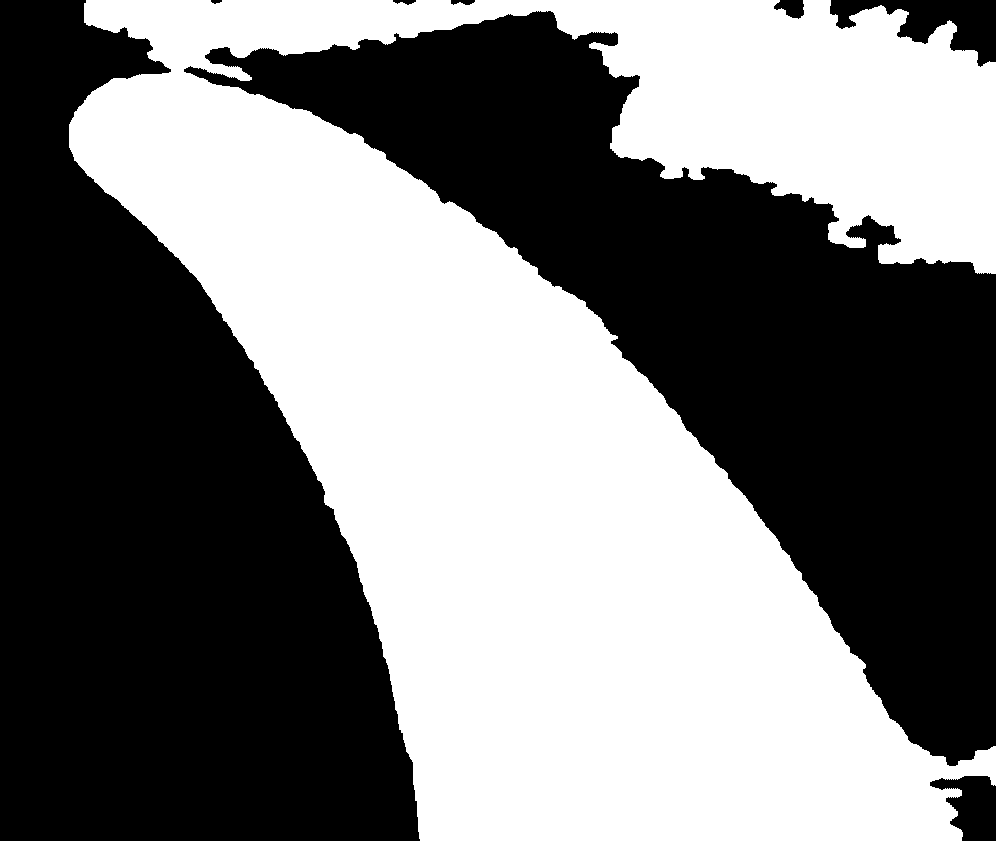
\includegraphics[width=\textwidth]{assets/images/alg_area/original.png}   
          \caption{Maschera originale}
        \end{minipage}
        \begin{minipage}{0.3\textwidth}
          \centering
          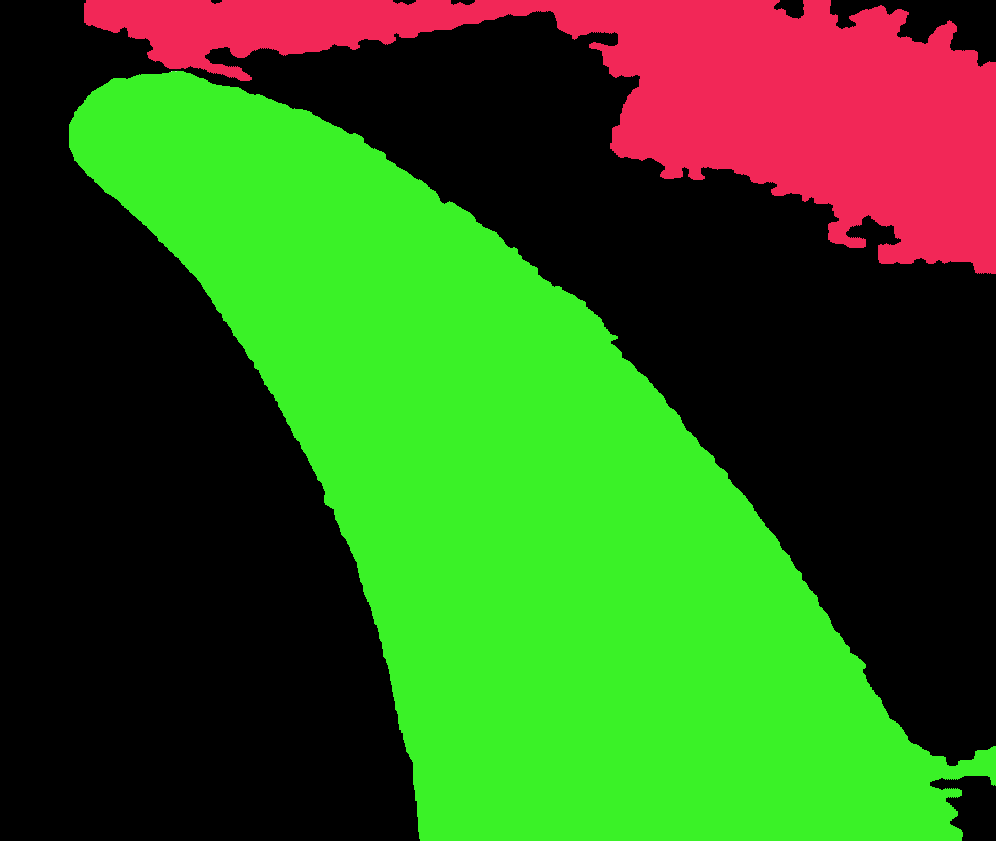
\includegraphics[width=\textwidth]{assets/images/alg_area/find.png}  
          \caption{Divisione in segmenti}
        \end{minipage}
        \begin{minipage}{0.3\textwidth}
          \centering
          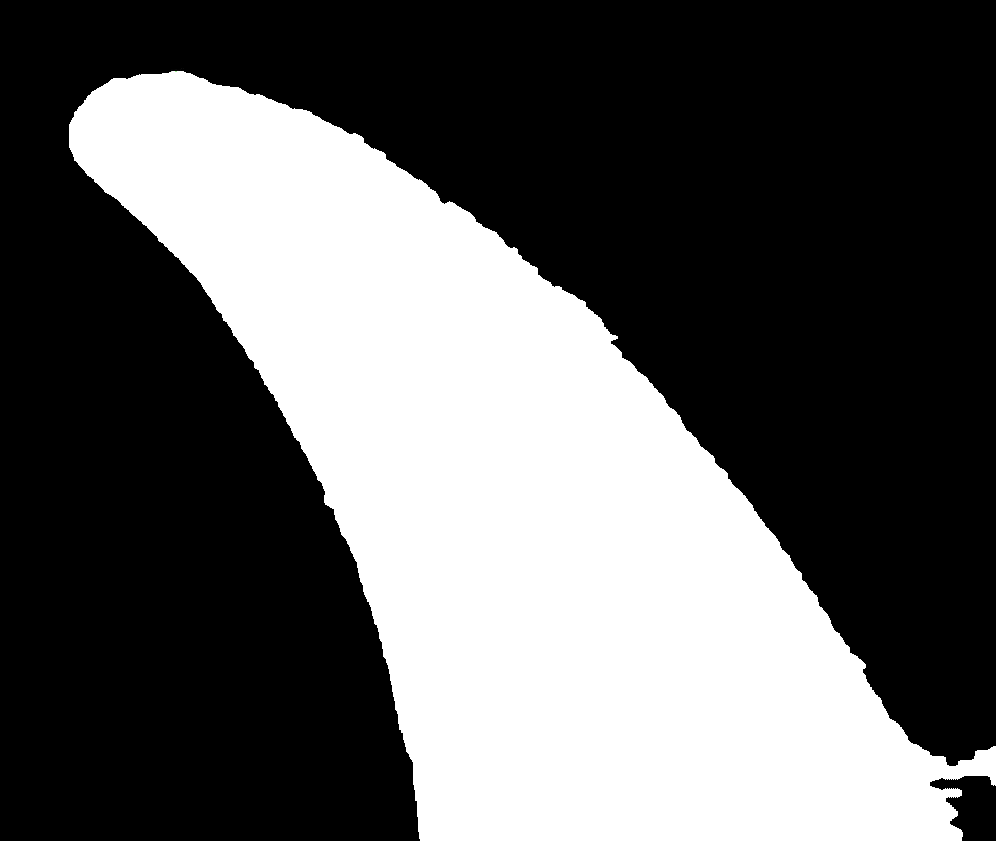
\includegraphics[width=\textwidth]{assets/images/alg_area/clear.png}   
          \caption{Rimozione segmenti minori}
        \end{minipage}
      \end{figure}
     
      Per quanto riguarda l'eliminazione di segmenti non appartenenti all'area della pinna del delfino
      è stato scritto un semplice algoritmo che si basa sul trovare tutti i segmenti separati all'interno della maschera,
      cercare il maggiore in base all'area del segmento e poi rimuovere tutto il resto dalla maschera, 
      questa operazione viene ripetuta sia prima che dopo l'utilizzo degli operatori morfologici, con il fine di
      eliminare eventuali scarti dell'erosione o del metodo OTSU.
      
  
      
      \newpage
      \begin{lstlisting}
#Trova i contorni nell'immagine binaria
contours, _ = cv2.findContours(im_thr, cv2.RETR_TREE, cv2.CHAIN_APPROX_NONE)

biggest_area = -1;
biggest = None;

for contour in contours:
    #Viene calcolata l'area del contorno
    area = cv2.contourArea(contour);

    #Salvataggio del contorno con l'area maggiore
    if biggest_area < area:
        biggest_area = area;
        biggest = contour;

#Disegno la maschera del contorno maggiore sulla maschera originale con una tonalità di grigio diversa
mask_colored = cv2.drawContours(im_thr, [biggest], -1, 80, -1);
_, binary_image = cv2.threshold(mask_colored, 254, 255, cv2.THRESH_BINARY_INV)

#Estraggo la maschera del contorno maggiore
mask = cv2.bitwise_and(mask_colored, mask_colored, mask=binary_image)

kernel = cv2.getStructuringElement(cv2.MORPH_ELLIPSE, (5,5))

#Applico operatori morfologici per eliminare eventuali buchi nella maschera
mask = cv2.morphologyEx(mask, cv2.MORPH_DILATE, kernel=kernel, iterations=1)
mask = cv2.morphologyEx(mask, cv2.MORPH_CLOSE, kernel=kernel, iterations=1)

#Altra Rimozione dei segmenti
#...
#Applico la maschera all'immagine originale per estrarre la pinna
fin = cv2.bitwise_and(image, image, mask=mask)
      \end{lstlisting}
      
    \subsection{Backend SPIR}
    dsad
    \subsection{Estrazione della maschera e della pinna del delfino}
    \subsection{Estrazione delle feature e salvataggio del dataset}
    \subsection{Match basato sulle feature estratte da SIFT}
    \subsection{Architettura del sistema}
    
  \section{Approccio basato su OpenCV per l'estrazione delle maschere}
    \subsection{Miglioramenti apportati al processo di ritaglio}
    \subsection{Parallelismo e tempi di esecuzione ridotti}
    \subsection{Riduzione dello spazio occupato dal dataset di feature estratte}
    \subsection{Adozione di gRPC per il trasferimento dei dati}
  \section{Approccio con deep learning per l'estrazione delle maschere}
    \subsection{Implementazione di una rete neurale basata su U-Net}
    \subsection{Utilizzo delle maschere per il ritaglio della pinna}
  \section{Interfaccia utente e interazione}
    \subsection{Creazione di un'interfaccia per l'interazione con il backend Python}
    \subsection{Utilizzo di Flutter per sviluppare un'interfaccia multipiattaforma}

\chapter{Risultati sperimentali}
  \section{Valutazione dei risultati}
    \subsection{Confronto tra i diversi approcci implementati}
    \subsection{Analisi delle prestazioni e dei risultati ottenuti}
  \section{Limitazioni e problematiche riscontrate con approccio Deep Learning}

\chapter{Conclusioni}
  \section{Riepilogo degli obiettivi raggiunti}
  \section{Possibili sviluppi futuri}

\chapter{Codice sorgente}
  \section{Implementazione dell'algoritmo SPIR}
  \section{Implementazione della rete neurale U-Net}
  \section{Codice per l'estrazione delle maschere con OpenCV}
  \section{Codice per l'interfaccia utente in Flutter}

\end{document}